\section{Tensor Transformations}
% Authors: Dustin Godevais , Reuben Juste, Yi Li,. 2/5/18.

The following sections summarize and visualize how you can transform data represented in matrix form. 
Input data can be defined as a matrix with the $i^{th}$ row corresponding to the $i^{th}$ data point and each additional columns representing a new dimension of the data.
$\matr{X}$ in the below examples is an input matrix with 1000 data points and two dimensions whose values are standard normally distributed. 
In the following figures, data points are colored according to their original $x_{N,1}$  dimension violet to yellow for negative to positive values.

\[
\matr{X} =
\begin{bmatrix}
    x_{1,1} & x_{1,2} \\
    x_{2,1} & x_{2,2} \\
    x_{3,1} & x_{3,2} \\
    \vdots & \vdots  \\
    x_{1000,1} & x_{1000,2}
\end{bmatrix}
\]

\begin{figure}[h]
\begin{center}
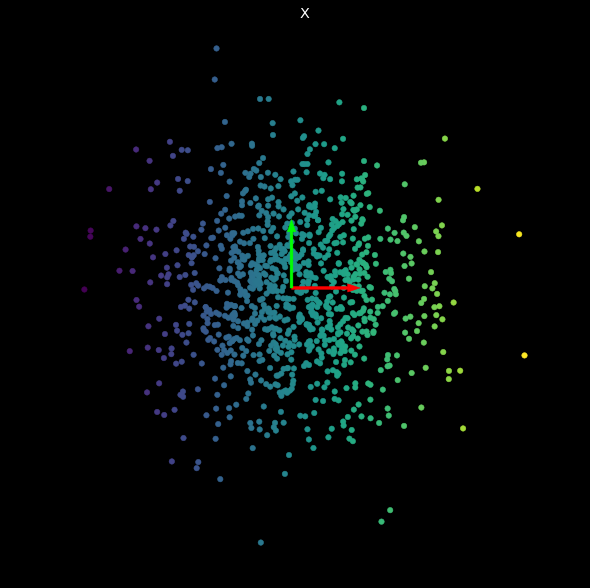
\includegraphics{labs/01/images/standardnormal.png}
\end{center} 
\caption{Original $\matr{X}$ Visualized}
\label{fig:mon}
\end{figure}

\subsection{Linear Transformations}
% Authors: Dustin Godevais , Reuben Juste, Yi Li,. 2/5/18.
There are several linear transformation that can be executed on $\matr{X}$ including:

\begin{itemize}
% \tightlist
\item
Rotation (\(\matr{U}\))

\item
Scaling \((s_1, s_2)\)

\item
Reflection (\(\matr{V}\))
\item
Shearing
\item
Translation
\end{itemize}

The product of the first three form weights as shown below.

\[
\matr{W} = \matr{U}
\begin{bmatrix}
    s_1 & 0 \\
    0 & s_2 
\end{bmatrix}
\matr{V}^\top
\]


\subsubsection{Rotation}
During rotation, each point is rotated about the origin by the indicated angle. 
The below equation populates $\matr{U}$ based on rotating points by \(\theta\) counter-clockwise.

\[
\matr{U} = 
\begin{bmatrix}
    \cos(\theta) & \sin(\theta)\\
    \sin(\theta) & -\cos(\theta)
\end{bmatrix}
\]

Keeping scaling and reflection constant, the below figure shows a set up points with different  \(\theta\)s .

\begin{figure}[h!]
\begin{center}
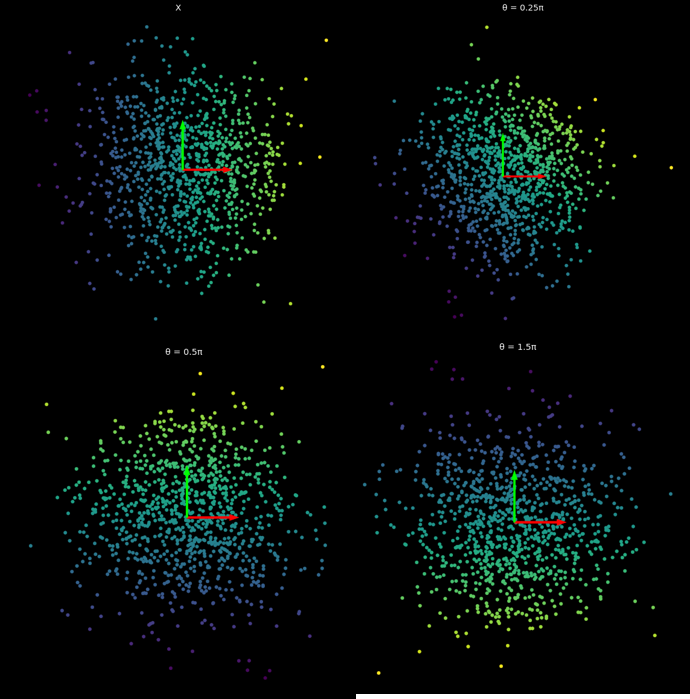
\includegraphics{labs/01/images/Rotation.png}
\end{center} 
\caption{Rotation Visualized}
\label{fig:mon}
\end{figure}
% \FloatBarrier


\subsubsection{Scaling}
Scaling the points expands or contracts the points about the origin. 
This controlled separately for each dimension by \(s_1\) and \(s_2\) .

\begin{figure}[h!]
\begin{center}
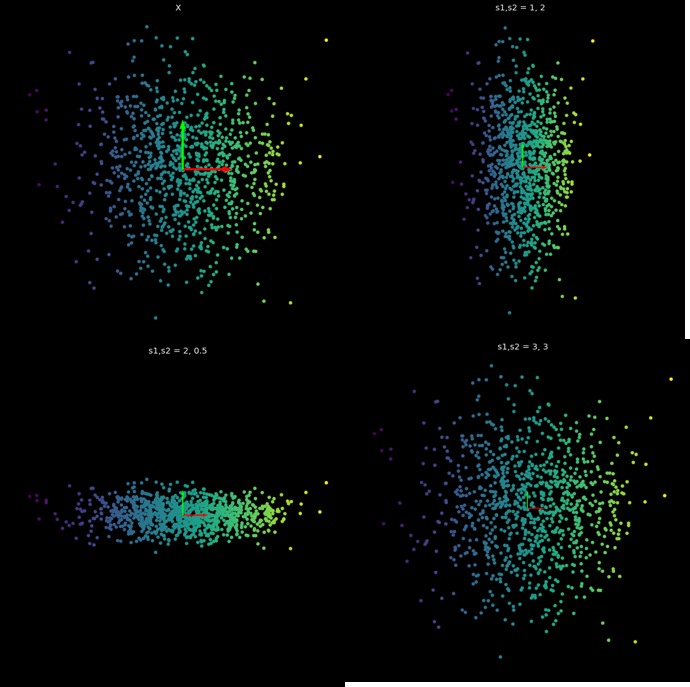
\includegraphics{labs/01/images/Scaling.png}
\caption{Scaling Visualized}
\label{fig:mon}
\end{center} 
\end{figure}
% \FloatBarrier


\subsubsection{Reflection}
Reflecting points projects them on the other side of a defined line that crosses the origin. 
The line that goes from the original point to the projected point is perpendicular to the defined line, and the intersection to the defined line is the midpoint.


\begin{figure}[h!]
\begin{center}
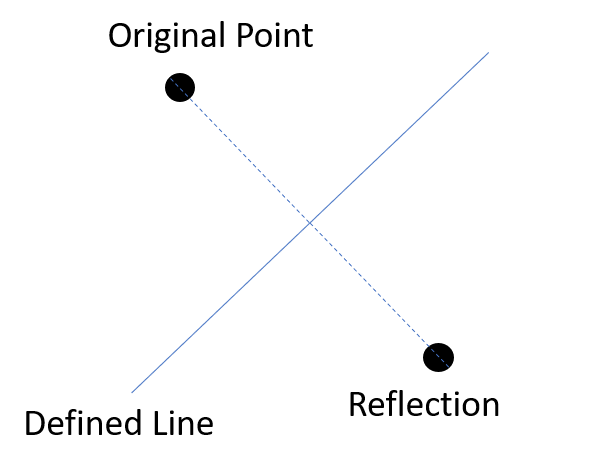
\includegraphics{labs/01/images/reflection_example.png}
\end{center} 
\caption{Reflection Defined}
\label{fig:mon}
\end{figure}
% \FloatBarrier


\(\matr{V}\) can be defined by

\[
\matr{V} = 
\begin{bmatrix}
    \cos(2\theta) & \sin(2\theta)\\
    \sin(2\theta) & -\cos(2\theta)
\end{bmatrix}
\]

Where the defined line is \(x_2 = \tan(\theta) x_1 \)

\begin{figure}[h!]
\begin{center}
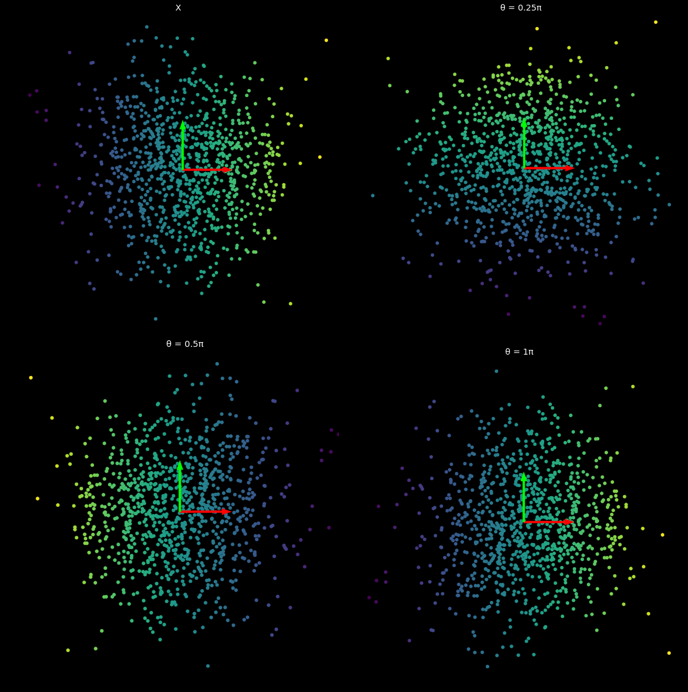
\includegraphics{labs/01/images/Reflection.png}
\end{center} 
\caption{Reflection Visualized}
\label{fig:mon}
\end{figure}
% \FloatBarrier

\subsubsection{Shearing}
Shearing points, which is separate from the weight calculation, shifting points in one dimension proportional to their value in the other dimension.

\(\matr{Y} = \matr{X}  \begin{bmatrix}
    1 & k\\
    0 & 1
\end{bmatrix} \) 
Shift points on the \(x_1\) dimension proportional to the \(x_2\) dimension

\(\matr{Y} = \matr{X}  \begin{bmatrix}
    1 & 0\\
    k & 1
\end{bmatrix} \)
Shift points on the \(x_2\) dimension proportional to the \(x_1\) dimension

\begin{figure}[h!]
\begin{center}
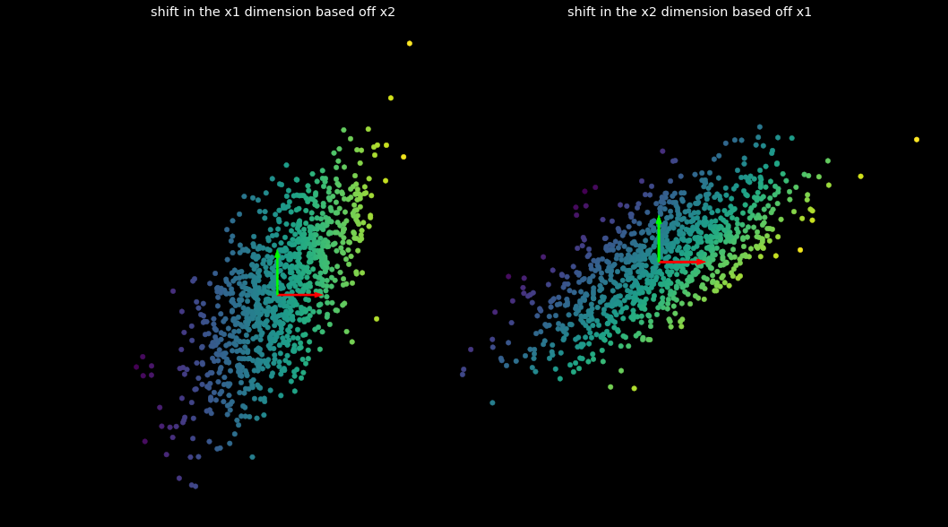
\includegraphics{labs/01/images/shear.png}
\end{center} 
\caption{Shear Visualized}
\label{fig:mon}
\end{figure}
% \FloatBarrier

\subsubsection{Translation}
The translation of points, which is separate from the weight calculations moves them uniforming in the direction indicated.

\[ \matr{Y} = \matr{X} 
+ \begin{bmatrix}
    1 & 1 \\
    1 & 1 \\
    1 & 1 \\
    \vdots & \vdots  \\
    1 & 1
\end{bmatrix}
\begin{bmatrix}
    t_1 & 0\\
    0 & t_2
\end{bmatrix} \] 
(Shift points left or right by \(t_1\) and up or down by  \(t_2\) dimension)

\begin{figure}[h!]
\begin{center}
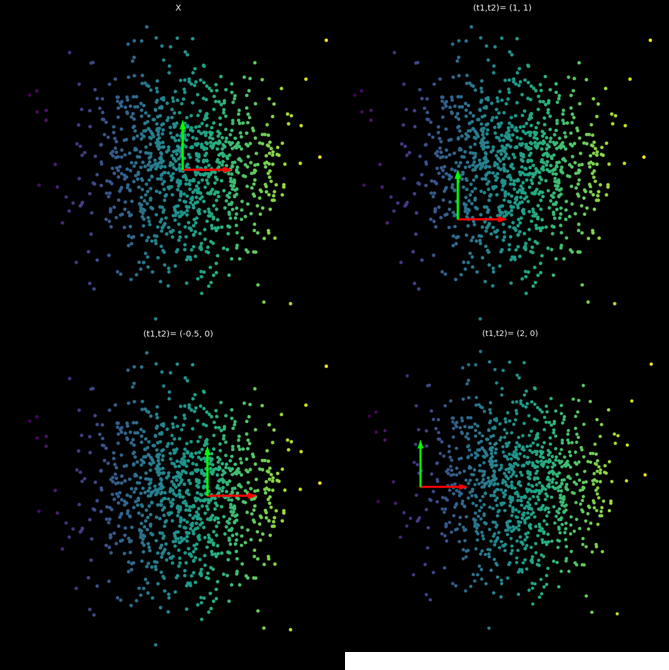
\includegraphics{labs/01/images/translation.png}
\end{center} 
\caption{Translation Visualized}
\label{fig:mon}
\end{figure}
% \FloatBarrier

\subsection{Non-Linear Transformations}
% Authors: Dustin Godevais , Reuben Juste, Yi Li,. 2/5/18.
Linear transformations are capable of altering data in many different ways, but linear transformations cannot curve data. 
That is where non-linear transformations come in. There are several types of non-linear transformations such as:

\begin{itemize}
% \tightlist
\item
Rectified linear unit (ReLU) - \(y = x_1\) if \(x_1 > 0\) else $0$ 
\item
Polynomial- \(y = x_1^2\) or \(y = x_1 x_2\)
\item
Step - \(y = 1\) if \(x > 0 \) else $0$ 

\end{itemize}

One of the most common non-linear transformations is the hyperbolic tangent, which in the context of 2D Tensors can be applied as below:
\[f(x) = \tanh(
\begin{bmatrix}
s & 0\\
0 & s
\end{bmatrix}
x)\]

This function first stretches out the points using scalar $s$ via \hyperref[subsubsec:Scaling]{scaling}, then tanh squashes the points into a square.
The larger $s$ is, the more points end up in the square.

\begin{figure}[h!]
\begin{center}
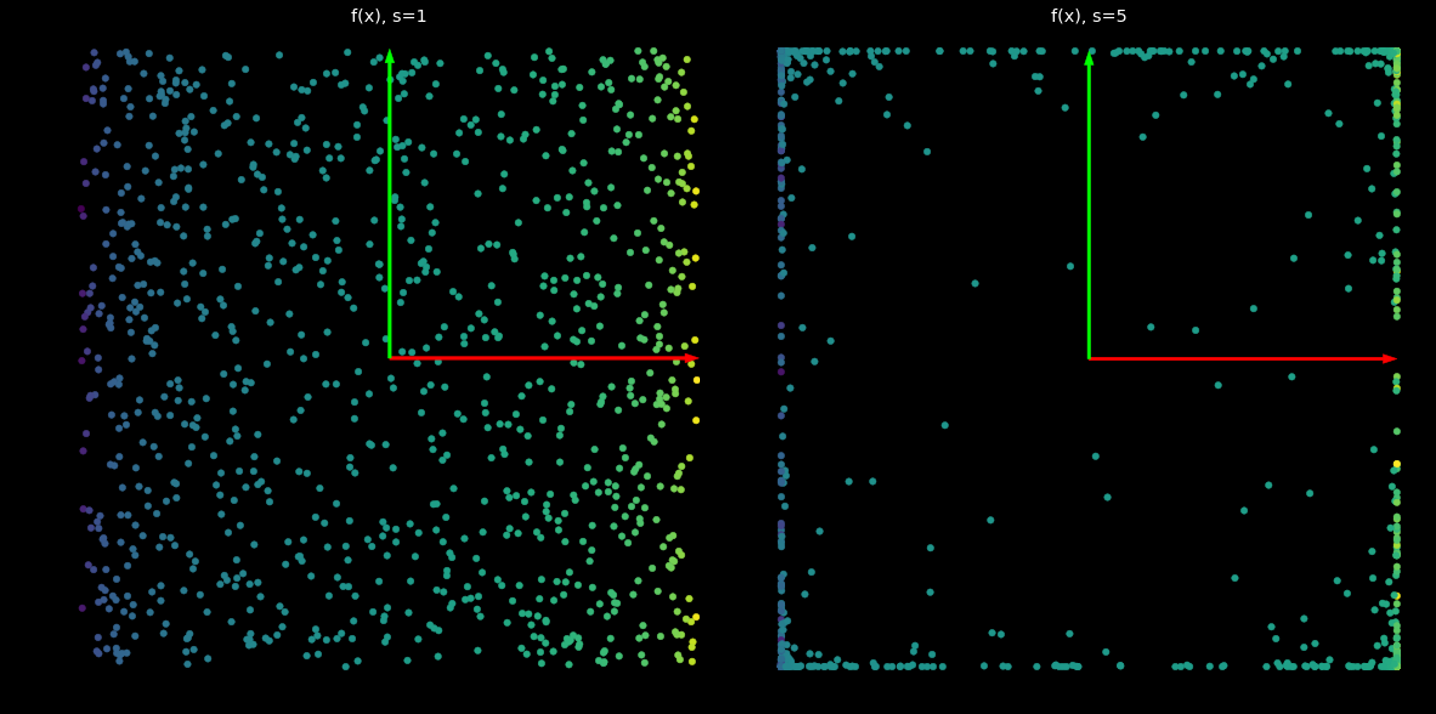
\includegraphics{labs/01/images/tanh.png}
\end{center} 
\caption{Tanh in Isolation}
\label{fig:mon}
\end{figure}
% \FloatBarrier

Tanh can create curved surfaces when it is sandwiched in-between two linear transformations in a three layer neural network.

\begin{figure}[h!]
\begin{center}
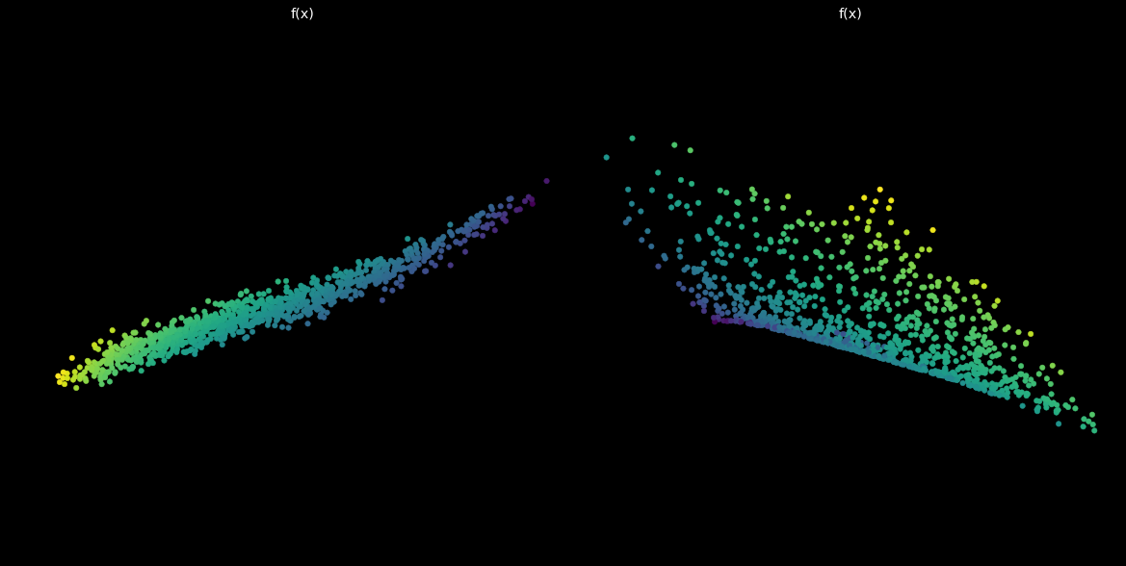
\includegraphics{labs/01/images/tanh_sandwich.png}
\end{center} 
\caption{Tanh In-Between Two Linear Layers}
\label{fig:mon}
\end{figure}
% \FloatBarrier
